\label{ch:fem}
As a conclusion of the previous chapter one can see that the number of methods that are currently available to describe a free electron function in presence of an intricate electrostatic background potential is not that large.
In this work the method of choise to model the free electron function is the FEM which had been applied to quantum mechanical problems already by several authors \cite{fem_hydro, vib_fem, fe_hf, fe_dft1}, however, to the best of my knowledge, only to bound state problems so far.
A brief review about these works is given in section \ref{ch:feQM}.
Besides its large flexibility and computational efficiency pointed out in section \ref{ch:introFEM} already, the large amount of available libraries for FEM \cite{libmesh,dealII,freefem, hermes,oofem} is another advantage of practical importance due to the complexity of the generation of a suitable mesh, assembling of matrices and solution of matrix equations.

In the following chapter the integration of the matrix elements (section \ref{ch:feInt}) and set up of the mesh (section \ref{ch:feAss}) will be described.
Thereby the focus is put on the application to the one-particle SE that is to be solved with molecular electrostatic potential.
Since the interest thereby is on free particle solutions, the spectrum is expected to be very dense and the wave function to be delocalised, requirering for well-designed boundary conditions.
A discussion of various boundary conditions and asymptotic descriptions available for FEM is described in section \ref{ch:BC}.

\section{Finite Element Calculations in Quantum Chemistry}
\label{ch:feQM}
The FEM is mainly known from engineering disciplines where it is used in a broad range of applications such as modelling of fluids \cite{fluid1,fluid2}, heat transfer and flow \cite{heat1, heat2,heat3} or material deformation under mechanical stress \cite{deform1, deform2}.
However, also several different quantum chemical problems have been solved with this method: SE solvers for small systems such as light atoms \cite{fem_hydro,fem_He,fem_He1, fem_h1, LiGS_fem} or diatomics \cite{fem_H_refine}, vibrational model systems \cite{vib_fem} and solid state problems \cite{fem_crystal, fem_crystal1}.
Moreover, even Hartree-Fock \cite{fe_hf} and DFT calculations on systems up to the size of benzene \cite{fe_dft1, fe_dft2, fe_dft3} have been performed, yielding results comparable to those obtained by the usual linear combination of atomic orbitals (LCAO) approach.

The above-mentioned publications have shown that the FEM is able to obtain reasonable results for molecular systems where the errors were comparable to those obtained with standard quantum-chemistry schemes even though their computational costs are higher.
This suggests that the FEM is a good tool for computations in the field of quantum chemistry for going beyond the capabilities of the established schemes such as the description of unbound states.

%\section{From Weak Form to a Matrix Equation}
\section{Integration of Matrix Elements and Formulations of the Equation System}
\label{ch:feInt}
In section \ref{ch:introFEM} the basics of the FEM were described and the generalised eigen system shown in eq. (\ref{eq:SEmat}) to solve the SE was derived.
Here this is taken as starting point and a closer look at the computation of the matrix elements as well as solving strategies for the large sparse generalised eigen problems are taken.

The generalised eigenproblem as given in eq. (\ref{eq:SEmat}) consists of three matrices.
Since the ansatz functions (shape functions) $\varphi_i(\vec{r})$ have only a small support, most of the matrix elements are zero. 
However, in two and three dimensions no distinct band structure is achievable and the matrices are irreducible.
Thereby matrix elements are zero when the elements involved are not neighboured.
The computation of the non-zero matrix elements involve an integration as \textit{e.g.} the overlap integral $\mat{M}_{i,j}=\int d \vec{r} \varphi_i(\vec{r}) \varphi_j(\vec{r})$ of ansatz functions,.
Since these functions are the same for all elements, the evaluation of these integrals can be done via a lookup-table or an efficient numerical integration scheme whose required order is well-known and need only be multiplied by the Jacobian of the respective elements involved.
The matrix elements $\mat{A}_{i,j}=\int d \vec{r} \left(\nabla \varphi_i(\vec{r})\right)\left(\nabla \varphi_j(\vec{r})\right)$ consist similar to those of $\mat{M}$ of overlap integrals of known functions.
The only matrix containing system-specific information is the potential $\mat{V}_{i,j}=\int d \vec{r} \varphi_i(\vec{r}) V(\vec{r}) \varphi_j(\vec{r})$ which requires numerical integration by which $V(\vec{r})$ is approximated as a spline of given order.

After assembling the matrices the eigenpair $(e_i, \vec{c}_i)$ of the system
\begin{equation} \label{eq:SEmat2}
\left(\frac 12 \mat{A}+\mat{V}\right)\vec{c}_i = e_i \mat{M}\vec{c}_i
\end{equation}
need to be found where $e_i$ should be closest to the analytic value of the kinetic energy of the photoelectron.
Since matrix eigenvalue equations with several thousands of dimensions occur in many fields, numerous schemes have been developed to solve them efficiently \cite{davidson,arnoldi, gpusolver,krylov}, a selection of them is described in section \ref{ch:ghep}.
Despite the numerical complexity due to the high dimensionality of this problem (several thousands of basis functions) the second problem is due to the fact that the eigenenergies $e_i$ are expected to be close to each other since the corresponding analytical problem has a continuous spectrum in this range.
It is well known in numerics that this leads to instabilities especially for the eigen vectors, making a regularisation of the problem (described in section \ref{ch:regular}) indispensable.

\section{Element Types and Mesh Types}
\label{ch:feAss}
Among the FEM formulations several `flavours' were designed for different purposes.
Given a certain equation to be solved in FEM there are in general two systematic ways to increase the accuracy.
The first way is to increase the number of elements witch is referred to as the $h$-FEM approach \cite{dreyer,}.
The refinement of the mesh is in principle always possible but technically demanding since it is not known in which regions of a mesh are too coarse in general \cite{dreyer}.
To overcome this, some FEM implementations such as that of \prog{Libmesh} \cite{libmesh} which is used here, provide an adaptive mesh refinement scheme, iteratively refining the mesh using local error estimations and thus fully automatic \cite{libmesh}.
But theses schemes are numerically demanding and hence can be only applied to benchmark systems.

The second strategy is called $p$-FEM. 
In the $p$-FEM scheme, the order $p$ of the test functions in increased, resulting in smother and more flexible solutions.
This scheme requires a large set of functions to be implemented but is known to yield good results if the function is smooth \cite{p-fem}.
While standard FEM-libraries usually have only $p=1,2$ implemented, others have high-order polynomials implemented \cite{hermes}.
Combined schemes where the grid-size as well as the element order are adapted is referred to as $hp$-fem \cite{hp-fem}.

Besides these different refinement strategies, finite element types also vary in their use of the degrees of freedom.
While Lagrange elements are integrated by evaluating certain inner or boarder points, \textit{e.g.} in Argyris or Hsieh-Clough-Tocher elements also first or even second derivatives are evaluated \cite{femPraxis,femCiarlet}.
Moreover, the arrangement of elements one distinguishes conforming and the more general non-conforming meshes \cite{nonconfFEM}. In case of the latter, more general structures are supported as \textit{e.g.} hanging nodes which occur when a vertex of one element is on the edge of an other as can be found in Figure \ref{fig:HexBenz} \cite{femCiarlet}.
The setup of the mesh is, as mentioned above already, critical to the quality of the solution and hence of special importance.
Moreover, it is technically non trivial to set up a close packing of volume elements with the desired properties in a systematic way.
There are different element types available, each with their techniques for set up.
Although in principle any element shape can be chosen, in three dimensions only tetrahedral (simplex), prism- and pyramid-shaped as well as hexahedral elements commonly are used.
By choosing the element shape and the polynomial order, also the type of shape functions is defined.
%When using hexahedral elements the ansatz functions usually are of the type $\varphi(\vec{r})=x^ky^lz^m$ where $p=k+l+m$ is the element order.

When considering meshes to describe molecular properties it is clear that the element size should be smaller in the vicinity of the nuclei while it may be broader at larger distances.
One way to create a hexahedral mesh with local refinement is to start with a coarse uniform lattice and subdivide the hexahedra where necessary as shown in Figure \ref{fig:HexBenz} for a benzene molecule.
Another way is to setup small regular cubic grids around the nuclei and expand them radially in boxes of growing size as shown in Figure \ref{fig:HexDia}.
These brick-shaped elements however have the disadvantages that the regular cube-like structures therein might be not well-suited for atoms and molecules that rely rather on spherical shapes.
%Further hexahedral elements are known to give less accurate solutions than tetrahedra which are commonly used nowadays \textcolor{green}{cite}.

%\begin{wrapfigure}{r}{\textwidth}
%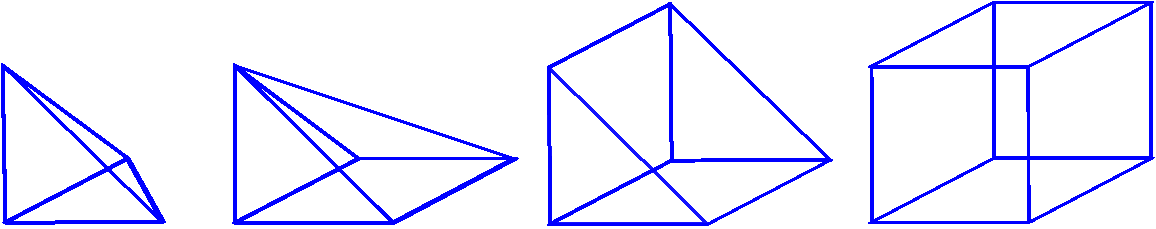
\includegraphics[width=\textwidth]{Figures/Elements3d-crop.pdf}
%\caption{The different Shapes of 3D elements.}
%\end{wrapfigure}
Another approach used by Lehtovaara \textit{et al.} \cite{fe_dft2} is to put layers of polyhedra around the atoms with increasing number of points and radii.
Thereby the overlapping regions of these spheres are removed by deleting elements that are closer to another atom.
\begin{figure}
   \begin{subfigure}{0.24\textwidth}
   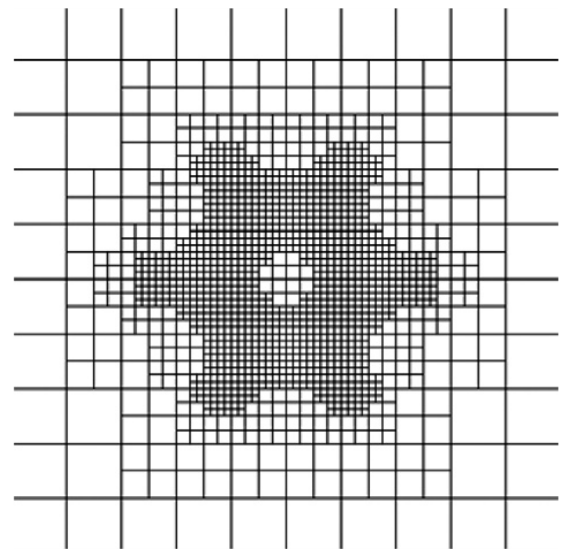
\includegraphics[width=0.95\textwidth]{Figures/QuadMeshBenzene}
   \caption{}
   \label{fig:HexBenz}
  \end{subfigure}
  \begin{subfigure}{0.24\textwidth}
   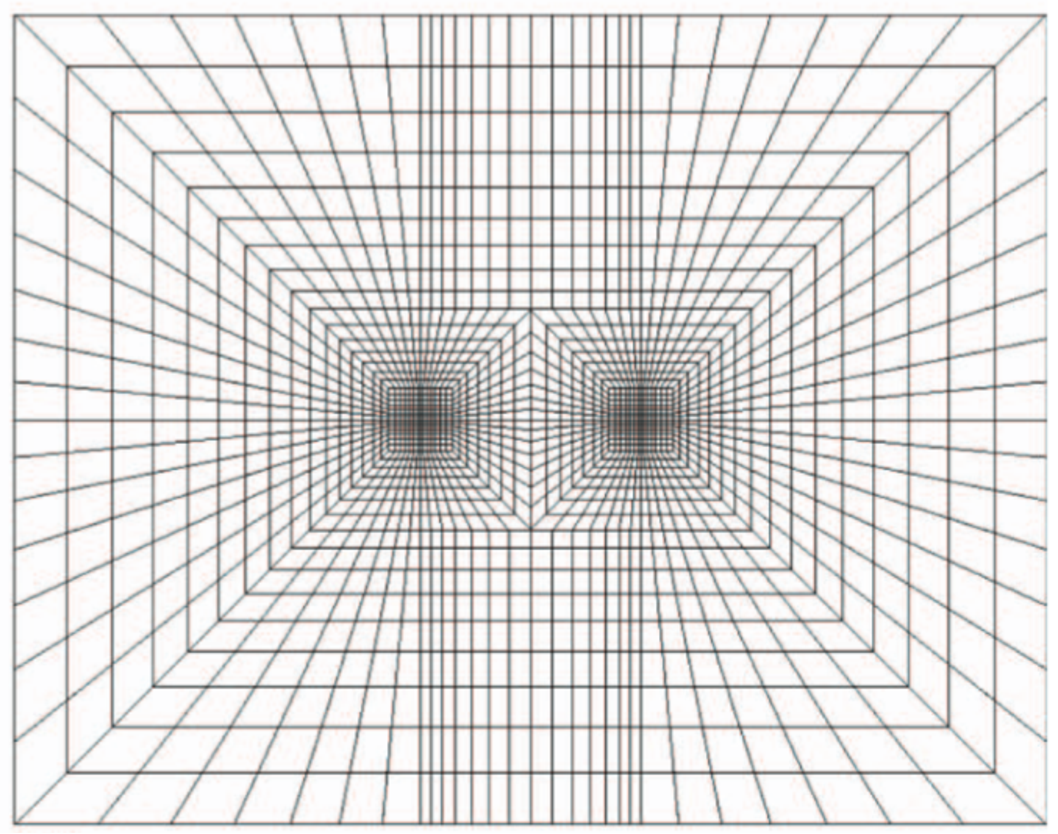
\includegraphics[width=0.95\textwidth]{Figures/QuadDiatomic}
   \caption{}
   \label{fig:HexDia}
  \end{subfigure}
  \begin{subfigure}{0.24\textwidth}
   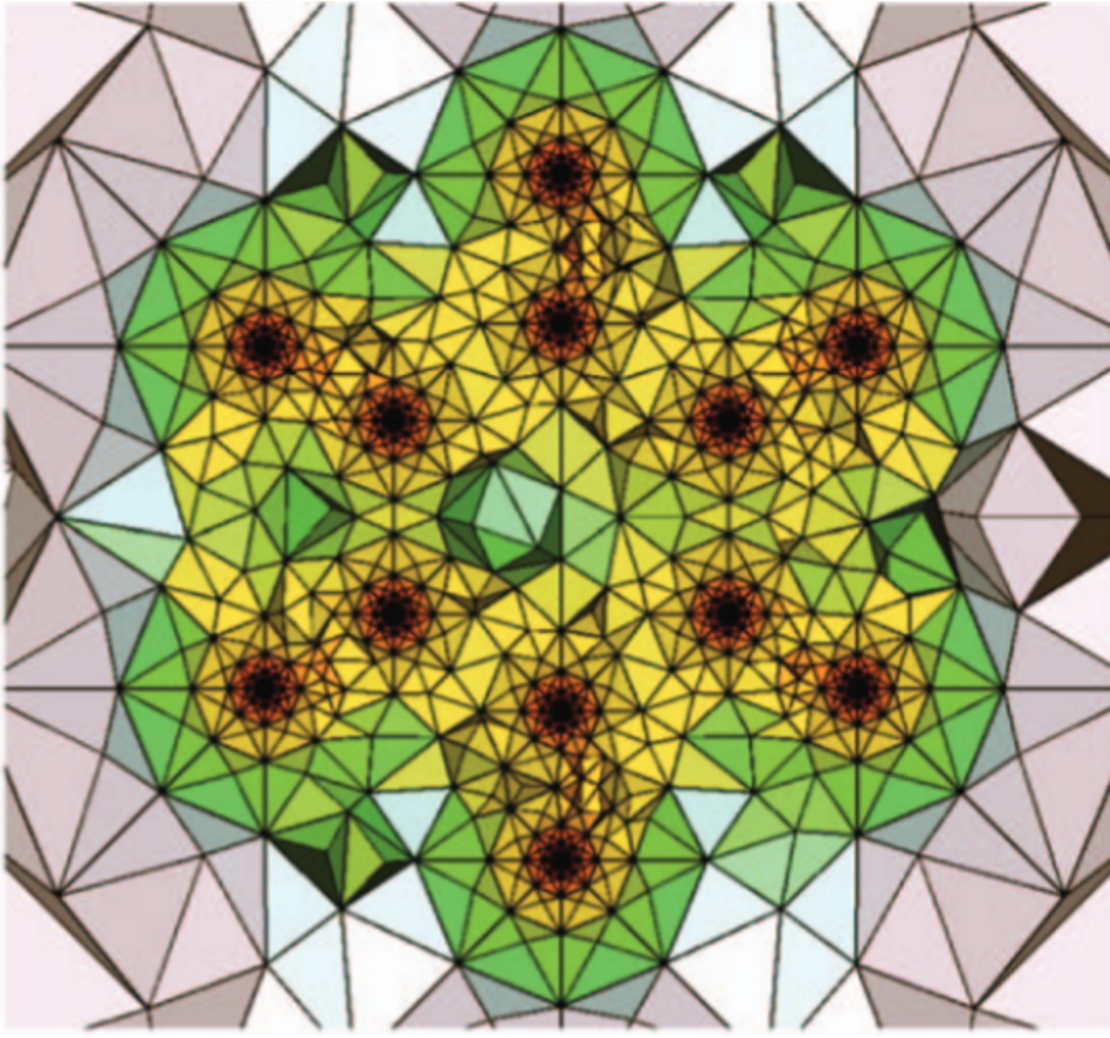
\includegraphics[width=.95\textwidth]{Figures/PolyBenzene}
   \caption{}
   \label{fig:PolyBenz}
  \end{subfigure}
  \begin{subfigure}{0.24\textwidth}
   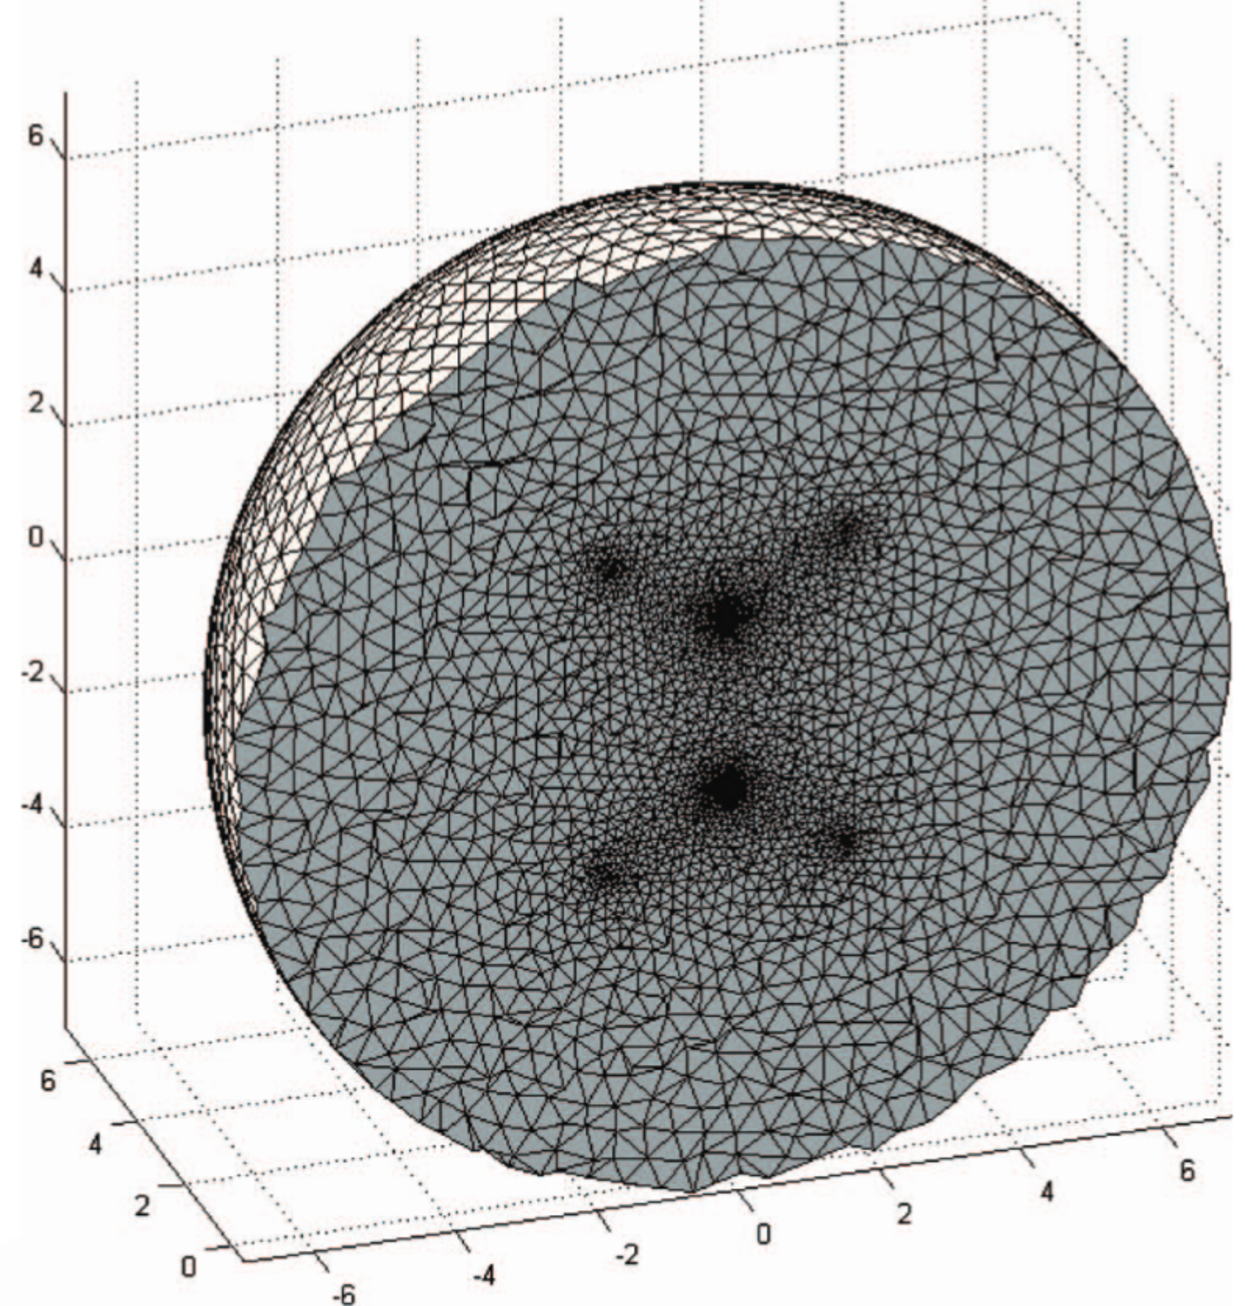
\includegraphics[width=.95\textwidth]{Figures/AdaptiveEthylene}
   \caption{}
   \label{fig:AdapEthyl}
  \end{subfigure}
  \caption{2D cuts through 3D meshes for molecular systems obtained with different schemes for local refinement:
    (a) hexahedral elements adapted for the benzene molecules \cite{fe_dft1}
    (b) hexahedral mesh for a diatomic \cite{fe_hf}
    (c) Polyhedral mesh for a benzene geometry \cite{fe_dft2}
    (d) Adaptive refined tetrahedral Mesh for ethylene. \cite{fe_hf}
    }
\end{figure}
The mesh obtained with this procedure for a benzene molecule \cite{fe_dft1} is shown in Figure \ref{fig:PolyBenz}.

When restricting oneself to tetrahedral elements, other design principles are possible: Since they are simplexes in three dimensions, they can be designed from general grids using \textit{e.g.} Voronoi \cite{voronoi} or Delaunay \cite{delaunay} tessellations (the latter is described in section \ref{app:delaunay} in appendix) from a set of points with the required properties.
Son and Chu \cite{Son_Chu, Son_Chu0} constructed sets of points resembling molecular geometries by inserting $N$ spherical grids with different radii $r_i$ around the atoms and cutting off the overlapping regions.
Thereby the respective radii are chosen as
\begin{equation}
r_i=\frac{il}{N-i+\frac{lN}{r_\text{max}}} \qquad i=1,\hdots ,N 
\end{equation}
where$r_\text{max}$ is the radius of the largest sphere and $l$ is a parameter smoothly changing between a linear $l\rightarrow \infty$ and a $1/r$-mapping.
As spherical grids they suggested the use of Lebedev-grids \cite{lebedev} and a design of Womersley \cite{Womersley2001,Sloan}.
A more detailed discussion about the choices of grids will be given in section \ref{sec:grid}.
%Choises for angular and radial grid distributions in this scheme are discussed in.% the chapters \ref{app:Sphere} and \ref{app:radius} respectively.

A more entangled method is used by Alizadegan \textit{et al.} \cite{fe_hf}. 
They start with an initial guess for the wave function and create a grid whose distances are inverse proportional to the second gradient of the electron density
\[
d \propto \left[ max\left\{\left|\frac{\partial^2 \rho}{\partial^2 x}\right| ,
                           \left|\frac{\partial^2 \rho}{\partial^2 y}\right| ,
                           \left|\frac{\partial^2 \rho}{\partial^2 z}\right| \right\} \right]^{-1}.
\]
which gives an estimate for the error due to linear approximation within each element.
After solving the eigenvalue equation on this grid, they recompute another mesh on the basis of the new function, iterating this procedure several times.
A cut through a mesh obtained by this procedure is shown in Figure \ref{fig:AdapEthyl}.

\section{Boundary Conditions}
\label{ch:BC}
Boundary conditions have not been addressed in this thesis so far for any of the methods but play an important role for the properties of the solution.
Hence there is a large number of boundary conditions.
The simplest case applicable here are Dirichlet-boundaries, requiring the wave function to vanish at the boundaries of the finite element box.
In the FEM this condition can be applied especially simple by setting the coefficients of the outermost shape functions to zero.

Due to the large extend of the free particle, these boundaries however are unphysical if they are not applied at distances that are several times larger than the wavelength.
However, considering a particle with $0.1\,$eV kinetic energy, its wavelength is $~4.4\,$Angstroms and the box would need to have a diameter of several tens of Angstroms which is not feasible any more while kinetic energies in the $m$eV-range would lead to even worse scenarios.

%These considerations make clear that a more advanced boundary condition is needed which has only local influence on the wave function.
%In the following sub chapters, three boundaries that can be applied in FEMs are introduced and discussed.
Besides the numerical restriction to a finite box also mapping schemes can be used as \textit{e.g.} $x=\tan (\frac y2)$ that maps $[-\infty:\infty]$ to $[-\pi:\pi]$ \cite{PSbook}.
However, using such a mapping directly is infeasible since the oscillations of the wave function would become arbitrarily sharp in the mapped range and hence the representation of the FEF would still be poor.

\subsection{Complex Absorbing Potential}
\label{ch:cap}
The complex absorbing potential (CAP) is a method often found in the literature when describing particles with infinite extent\cite{bauch1, bauch2}.
In this scheme, an artificial potential usually of the form
\begin{equation}
   W_\text{CAP}(\vec{r})=\begin{cases} i\nu(\vec{r}-\vec{r}_0)^2 & \vec{r}>\vec{r}_0 \\
                                           0    & \text{else} \end{cases}
\end{equation}
is added where $\vec{r}_0$ is larger than the bound part of the system.
Such a potential damps the reflection of the wave function at the boarders and thus enhances the quality of states obtained on a finite region \cite{cap1, cap2}.
However, studies with different shapes of these potentials show that it influences the wave function not only close to the boarders and a proper design of the parameters is non-trivial \cite{CAPfreshlook}.

To minimise the error due to the CAP, the parameter $\eta$ can be chosen such that its dependency on the energy vanishes in first order, \textit{i,e.} $\eta\frac{dE}{d\eta}=0$ \cite{CAPccEOM,CAPfreshlook}.
Moreover, due to non-hermiticity the usual scalar product is not suitable when calculating overlap integrals any more.
Too strong $\eta$ introcudes reflections, too weak $\eta$ lead to unstable resonances, making them strongly basis-set dependent \cite{CAPfreshlook}.
Moreover, for Helmholtz problems, a dependence of the error on the frequency was observed \cite{babuska}.

The idea of damping down a function and making sure no reflections are scattered back to the region of interest is common to further approaches as \textit{e.g.} absorbing boundary conditions \cite{Engquist}, transparent boundaries \cite{HelmhPrec}, perfectly matched layer schemes \cite{pmlBook,pml1, pml2} or certain variable transformations \cite{taoDVR}.

\subsection{Mode-matching Schemes}
Consider the solution in an inner and outer region as different variables following the equations
\begin{equation}
   \nabla^2\Psi_1 +V(\vec{r})\Psi_1-E\Psi_1=0 \qquad \nabla^2\Psi_2 -E\Psi_2=0 
\end{equation}
whereby the outer function needs to satisfy the Sommerfeld condition $r^\alpha \left(\frac{\partial \Psi_2}{\partial r} - ik \Psi_2  \right)\rightarrow 0$.
These equations are coupled by the conditions
\begin{equation}
\Psi_1=\Psi_2  \qquad \nabla \Psi_1 \vec{n}=\Psi_2 \vec{n}
\end{equation}
to ensure continuity of the solution and the gradient normal to the boundary \cite{AstleyMM}.
Thereby, the asymptotic behaviour of the outer function is ensured by taking basis functions that individually fulfil the condition and the boundaries enter the weak formulation since the application of Greens' theorem leads to an extra term.

The mode-matching scheme can be considered as a generalisation of the R-matrix approach in a finite element formulation.

\subsection{The Boundary Element Method}
The boundary element method (BEM) can be used as a self-standing method for solving partial differential equations using the weak formulation \cite{bemDai,bemCostabel}.
In its pure form, the BEM solves the problems using only conditions given at its boundaries that are connected to the volume properties via Greens' theorem, the Gauss-Ostrogradskii (divergence) theorem as well as Stokes theorem \cite{bemBook}.
Even though the BEM procedure suffers strongly from the restriction of being applicable only to linear systems for which a fundamental solution is known as well as the disadvantage of leading to dense, unsymmetric matrix equations \cite{bemCostabel} it has some popularity until these days \cite{bem1,bem2,bem3}.
But its main advantages come into play when being used with the FEM \cite{bem-fem} where the FEM can be used to obtain an accurate solution in the inner region and the boundaries are treated with the BEM.
Considering an unbound domain as, \textit{e.g.} the problem of the outgoing electron, the infinite domain $\Gamma$ can be divided into a finite region $\Gamma_i$ where the atoms electrostatic potential leads to ... and the remaining domain $\Gamma_o$ in which the time-independent SE reduces to the Helmholtz-problem whose fundamental solutions are well-known and thus the BEM is applicable \cite{bemCostabel, bettessBEM}.

\subsection{Infinite Elements}
The infinite element approach was developed in the 1980-ths for acoustical caluculations and is specificly designed for the Helmholtz equation and can be understood as a advancement of the BEM that is speciallised for the Helmholtz equation.
The general idea of the infinite elements is that the solution of the radial Helmholtz equation in spherical symmetry is well-known to be of the form
\begin{equation} \label{eq:infAnsatz}
 \Psi(r) = \left(\frac ar +\frac{b}{r^2} + \hdots \right) e^{ikr}
\end{equation}
where $k=|\vec{k}|$ is the absolut value of the momentum of the particle and the prefactors thus correspond to different angular momenta of the outgoing electron.
In the complete limit any function fulfilling the Sommerfeld radiation condition \cite{sommerfeldCond} can be represented.

To use this asymptotic information, in the infinite element region a layer of elements is set onto the outer surface of the finite element region in which the shape functions are of the form (\ref{eq:infAnsatz}).
To fulfill the continuity conditions, the front-face of these elements coincides with the outer face of the respective finite element. while their radial faces have ray-like edges with a common centre in the middle of the finite element region.

Over the decades several formulations of infinite elements were developed which each make an ansatz for the solution of the form
\begin{equation} \label{eq:Infansatz}
 \Psi(\vec{r}) = \varphi(\vec{r}) e^{ik(r-r_0)},
\end{equation}
where $\varphi(\vec{r})=f(r)\varphi_2(\vec{r})$ is a product of a transversal shape function $\varphi_2(\vec{r)}$ which is orthogonal to the radial direction $r$.
The function $f(r)$ is a multipole expansion \textit{i.e.} a polynomial in $\frac{r_0}{r}$ where Jacobi-polynomials turned out te be most stable \cite{dreyer_improved}.
The differences in the formulations are introduced by the test functions applied \cite{Astley}.
%An overwiev about different formulations is given in the references \cite{dreyer} and \cite{Astley}.

\subsubsection{Burnett Elements}
In the original Burnett formulation, the test functions are given in the form
\begin{equation} \label{eq:BUelem}
 \Phi(\vec{r}) = \varphi(\vec{r}) e^{-ik(r-r_0)}.
\end{equation}
In the literature, usually the sign in the exponent is changed due to the use of an other convention in the notation of the weak formulation \ref{eq:SEweak}.
Important is, however, that in the equation later on the test and ansatz functions enter both with same oscillatory factor, introducing oscillations with $e^{2ik(r-r_0)}$ in the Hamiltonian.
These oscillations make the Hamiltonian non-hermitian and introduce a strong dependence on the energy $E=\frac{k^2}{2}$.
Moreover it was found that this formulation can lead to numerical instabilities \cite{Astley} and a wrong asymptotic behaviour.

\subsubsection{Conjugate Burnett Elements}
To get rid of the oscillatory terms, a modification of the test functions applied was introduced such that, in the notation used within this thesis, the test functions coincide with the space of ansatz functions, having the form
\begin{equation}
 \Phi(\vec{r}) = \varphi(\vec{r}) e^{ik(r-r_0)}.
\end{equation}
An important disadvantage of this formulation is, however, that in this formulation integrals with infinite contribution arise.

\subsubsection{Asley-Leis Formulation}
To regularise the matrix elements, an additional damping is needed.
Since the ansatz function (\ref{eq:Infansatz}) should not be changed for physical reasons, Astley suggested to chose test functions of the shape
\begin{equation} \label{eq:ALelem}
 \Phi(\vec{r}) = D(r)\varphi(\vec{r}) e^{-ik\mu(r)}
\end{equation}
where in three dimensions $D(r)=\frac{1}{r^2}$ \cite{astley2}.
This choise of basis functions is done at the expense that the Hamiltonian (\ref{eq:FEMmatrix}) is not hermitian.

Even though the oscillating term $e^{ikr}$ cancels out, the Hamiltonian is energy dependent and thus the generalised eigenvalue problem (\ref{eq:SEmat}) formulated in chapter \ref{ch:introFEM} changes to
\begin{equation} \label{eq:SEinf}
\mat{A}\vec{c} +ik \mat{B}\vec{c}- k^2 \mat{C}\vec{c} =0 
\end{equation}
with
\begin{align} \label{eq:InFEMmatrix}
\mat{A}_{i,j}& =\int \left(V(\vec{r}) D(r) \varphi_i(\vec{r}) \varphi_j(\vec{r}) 
                 -\frac 12 D'(r) \varphi_i(\vec{r})\varphi'_j(\vec{r})
                 +\frac 12 D(r) \varphi'_i(\vec{r})\varphi'_j(\vec{r}) \right) d\vec{r}\\
\mat{B}_{i,j}&=\frac 12 \int\left( -\mu'(r)D'(r) \varphi_i(\vec{r})\varphi_j(\vec{r})
                + D(r) \left(\varphi'_i(\vec{r})\varphi_j(\vec{r}) -\varphi_i(\vec{r})\varphi'_j(\vec{r})\right) \right) d\vec{r} \\
\mat{C}_{i,j}&= \frac 12 \int\left( (D(r) \mu'(r) \mu'(r) + 1) D(r) \varphi_i(\vec{r}) \varphi_j(\vec{r})\right) d\vec{r}
\end{align}
where the prime is used as short-form of the spacial derivative and the relation $E=\frac 12 k^2$ is used \cite{dreyer}.

This reformulation though lead to a quadratic eigenvalue problem instead of the generalised eigenvalue problem from before.
However, assuming that the difference between the eigenvalues of (\ref{eq:SEinf}) and the target energy of the outgoing electron is small, the quadratic eigenvalue problem can be approximated by the generalised eigenvalue problem (\ref{eq:SEmat}) by setting $k$ to the respective target momentum in the Hamiltonian.
However, this approximation, which is applied here for simplicity, needs to be verified.

The nonhermiticity of this Hamiltonian is, however, an important drawback of this formulation.
The introduced imaginary part of the eigenvalue can be considered as a broadening of the line width and thus as a lifetime as well as an uncertainty of the energy.
However, this is not very meaningfull since the ansatz is done in praticular in such a way that the wave function is not changed in an unphysical sense.
To understand the respective results, here a symmetrised ansatz is suggested in the following.

\subsubsection{Symmetrised Formulation}
Besides those formulations mentioned above, further infinite element formulations are used \cite{dreyer}.
For example, a formulation to the Burnett-elements using a quadratic decay was applied to the harmonic oscillator \cite{bettessHarmonic} and DFT calculations \cite{sobaMolecule} successfully.
However, the application of infinite elements to FEFs is to my knowledge a novelty in this work.

Since the Astley-Leis elements suffer from their non-symmetric space of ansatz- and test-functions whereas the conjugate Burnett formulation has problems due to infinitely large matrix elements, here a symmetric but damped ansatz of the form
\begin{align} \label{eq:ALsymm}
\Psi(\vec{r}) &= D(r)^p\varphi(\vec{r}) e^{ik\mu(r)} \\
\Phi(\vec{r}) &= D(r)^p\varphi(\vec{r}) e^{ik\mu(r)}
\end{align}
is suggested where $\varphi(\vec{r})$ is of the form as before but $D(\vec{r})=\frac{1}{r^2}$ with $p>0$ ensures that the matrix elements are finite-valued.
The basis formulation (\eq{eq:ALsymm}) changes the mass and potential energy matrices only in a trivial way whereas the kinetic energy matrix, which is in the original Astley-Leis formulation non-hermitian, becomes now
\begin{multline}
\int \left(\nabla \Phi^*_i(\vec{r})\right) \left(\nabla \Psi_j(\vec{r})\right) d\vec{r}=
\int D^{2p}\left(
p^2 \frac{D'(r) D'(r)}{D^2(r)} +p \frac{D'(r)}{D(r)} \left(\varphi_i(\vec{r})\varphi'_j(\vec{r})+ \varphi'_i(\vec{r})\varphi_j(\vec{r}) \right)\\
+ \left(  \varphi'_i(\vec{r})\varphi'_j(\vec{r}) + ik\mu'(r) \left(\varphi_i(\vec{r})\varphi'_j(\vec{r})- \varphi'_i(\vec{r})\varphi_j(\vec{r})  \right) -(ik\mu'(r))^2 \varphi_i(\vec{r})\varphi_i(\vec{r}) \right)
\right)d\vec{r} 
\end{multline}

\section{Solving Large Eigenvalue Problems}
In finite element applications such as those being proposed in this work, matrix equations with hundreds up to hundredthousands of dimensions need to be solved.
This requries elaborate strategies, using the sparsity of these matrices.

The focus here is on solving the generalised eigenvalue problem (\ref{eq:SEmat}) and the quadratic problem (\ref{eq:SEinf}) respectively.
However, efficient strategies are only known for regular eigenvalue problems of the form 
\begin{equation} \label{eq:eigenprob}
\mat{A}\vec{x}=\lambda\vec{x}.
\end{equation}
Hence, the more general forms will be rewritten to become (\ref{eq:eigenprob}) as discussed in sections \ref{ch:GenEV} respectively.
Moreover, since the state of interest is a free state, one needs to expect a high density of states for an appropriate mesh. 
This, however, is a well-known problem in numerical methematics since almost degenerate eigenvalues are very sensitive to small perturbations and their respective eigenvectors even more.
Though section \ref{ch:regular} addresses these problems and a way for numerical stabilisation is sketched.

Finally in section \ref{ch:ghep} a few methos are presented showing how a small number of approximate eigenpairs can be obtained in a numerically efficient way from the usual eigenproblem (\ref{eq:eigenprob}).
% general overview: http://www.sciencedirect.com/science/article/pii/S0377042700004131

%How is this inversion done numerically?
%
%\subsection{Quadratic Eigenproblem}
%\label{ch:quadEV}
%--> Probably this chapter is not of interest here since I don't use the respective formulation!?

\subsection{Generalised Eigenproblem}
\label{ch:GenEV}
The most straight-forward way to reformulate the generalised eigenvalue problem
\begin{equation} \label{eq:Gep}
\mat{A}\vec{x}=\lambda\mat{B}\vec{x},
\end{equation}
is te invert the matrix $\mat{B}$, obtaining the regular Eigenproblem $\mat{B}^-1\mat{A}\vec{x}=\lambda\vec{x}$.
This way is possible as long as $\mat{B}$ is invertable and not too large since inversion is a demanding task and the resulting matrix is not sparse anymore \cite{slepcManual}.

To prevent the use of dense matrices, libraries often do not operate with the matrices themselves but rather with a set of vector on which these matrices act \cite{slepcManual}.
The most popular scheme of this kind is the Rayleigh-Ritz projection where the initial problem is approximated on a small subspace $\mathcal{V}_j=span \{\vec{v}_1,\hdots,\vec{v}_j\}$, spanned by appropriate vectors $\vec{v}_i$.

Projecting the original problem (\ref{eq:Gep}) onto this subspace yields the new system $\mat{\Sigma}_j \vec{s}=\theta\mat{\Theta}_j\vec{s}$ where $\mat{\Sigma}_j=\mat{V}_j^T\mat{A}\mat{V}_j$ and $\mat{\Theta}_j=\mat{V}_j^T\mat{B}\mat{V}_j$ respectively which is only of dimensionality $j$.
The matrix $\mat{V}_j$ is unitary with the rows $(\mat{V}_j)_i=\vec{v}_i$.
After solving this dense but small problem, the original eigenvectors can be approximated as $\vec{x}_j=\mat{V}_j\vec{s}_j$ and $\lambda=\theta_j$.
The obtained eigenpair is a good approximation to the actual one as long as the subspace $\mathcal{V}_j$ contains the respective solution or contains a vector which is at least close to it.
A commonly used approach the Krylov subspace.

\subsection{Stabilisation of Eigenproblems}
\label{ch:regular}
Independent of the efficiency and robustness of the eigensolver in use, seeking solutions of the SE for free particles means that eigenpairs are to be found whose energies are, if the numerical parameters are chosen well, very dense or even degenerate.
Unfortunately, dense-lying eigenvalues lead to numerical difficulties and especially the eigenvectors are known to be unreliable in this case.
In practice this means that the iterative schemes do not converge anymore, requireing a reformulation of the mathematical probelm.

One way to circumvent the instabilities in the original problem (\ref{eq:Gep}) is to reformulate it as a minimisation problem \cite{H2pDeCleva}.
Therefore eq. (\ref{eq:SEmat2}) is rewritten as $\left(\frac 12 \mat{A}+\mat{V} - E \mat{M}\right)\vec{c}_i = 0$ where $E$ is the target energy.
Since this will have most likely no unambiguous solution, one minimises the residuum
\begin{equation}
\text{min}_{||\vec{x}||=1}\left\{\left|\left|\left(\frac 12 \mat{A}+\mat{V}-E\mat{M}\right)\vec{x} \right|\right| \right\}.
\end{equation}
Using the $L_2$-norm, this equivalent to finding the smallest eigenvalue of
\begin{equation} \label{eq:SEmin}
\left(\frac 12 \mat{A}+\mat{V}-E\mat{M}\right)^\dagger
\left(\frac 12 \mat{A}+\mat{V}-E\mat{M}\right) \vec{x}_i = \theta \vec{x}_i
\end{equation}
where $\theta$ is a measure for the error in energy.
%To avoid the costly multiplication of two matrices, one can use  Hermiticity of the matrices and take compute the
%square root as
%\begin{equation} \label{eq:SEmin}
%\left(\frac 12 \mat{A}+\mat{V}-E\mat{M}\right)\vec{c}_i = \lambda \vec{c}_i
%\end{equation}
%which is a usual eigenvalue problem \cite{H2pDeCleva} and $\lambda$ with smallest absolute value is searched.
%
%Nonetheless, the latter formulation is only an approximation as the comparison of (\ref{eq:Gep}) and (\ref{eq:SEmin}) shows, the latter approximates the mass matrix$\mat{M}$ as unity $\mat{1}$.
%Furthermore, eq. (\ref{eq:SEmin}) still is expected to have a very dense spectrum and $\lambda$ is an interior eigenvalue so the initial problem is not expected to be solved in this approach.

Whereas eq (\ref{eq:SEmin}) is only an approximation to the original problem, it has the advantage that it is a quadratic expression.
Similar schemes which are, in contrast to that mentioned above, only reformulations of the original problem are often referred to as spectral transformations \cite{slepcManual}.
One example is the harmonic extraction, where the eigenvalues of original expression (\ref{eq:Gep}) are first shifted such that the target value is $0$, leading to the equation 
\begin{equation} \label{eq:Shift}
\left(\mat{A}-\tilde{\lambda}\mat{M}\right)\vec{x}=(\lambda-\tilde{\lambda})\vec{x}
\end{equation}
where $\tilde{\lambda}$ is the target value of the original problem.
Than, the equation is multiplied by $\mat{A}$, resulting in the problem 
\begin{equation}
\left(\mat{A}-\tilde{\lambda}\mat{M}\right)\left(\mat{A}-\tilde{\lambda}\mat{M}\right)\vec{x}=(\lambda-\tilde{\lambda})\left(\mat{A}-\tilde{\lambda}\mat{M}\right)\mat{M}\vec{x}
\end{equation}
which is observed to lead to faster convergence for Krylov-subspace methods \cite{slepcManual}.

Further spectral transformations are the spectral folding \cite{slepcManual} where the left and right side of equation (\ref{eq:Shift}) are squared respectively which often leads to higher stability but the squaring of eigenvalues leads to ambiguities with respect to the eigenvalues $\lambda$ of the original problem.
%Instead of the reformulation, here a regularisation of the problem used, applying the spectral transformation shift and invert.
%Starting thit the problem: $\mat{A}\vec{x}=\lambda\mat{B}\vec{x}$ where the eigenvalues closest to the target energy $\varepsilon$ are of interest, the spectrum can be shifted to a target energy of $0$ by
%\begin{equation}
%\left(\mat{A}-\varepsilon\mat{B}\right)\vec{x}=(\lambda-\varepsilon)\mat{B}\vec{x}
%\end{equation}
The scheme that turned out to be most beneficial for the matrices used in this work is the shift and invert scheme where the inverted problem of eq. (\ref{eq:Shift}), \textit{i.e.}
\begin{equation}\label{eq:stSI}
\left(\mat{A}-\tilde{\lambda}\mat{M}\right)^{-1}\mat{M}\vec{x}=\frac{1}{\lambda-\tilde{\lambda}}\vec{x},
\end{equation}
is solved. 
The formulation (\ref{eq:stSI}) has the advantage that the transformed eigenvalues $\frac{1}{\lambda-\tilde{\lambda}}$ are well-separated and on the extrema of the new spectrum, making the convergence faster and more stable \cite{str-7}.
A more generalised transformation is the Cayley-transform which has two parameters $\tilde{\lambda}$ and $\tilde{\tilde{\lambda}}$ and yields the usual eigenvalue problem
\begin{equation}
\left(\mat{A}-\tilde{\lambda}\mat{M}\right)^{-1}\left(\mat{A}+\tilde{\tilde{\lambda}}\mat{M}\right)\vec{x}=\frac{\lambda+\tilde{\tilde{\lambda}}}{\lambda-\tilde{\lambda}}\vec{x}.
\end{equation}

Finally, a regularisation of eigenvalue problems can be performed using matrix preconditioners.
Many different types of preconditioners are developed \cite{Helmke2010} but most of them are effective only on a small class of problems as \textit{e.g.} especially well-suited for matrices originating from FEM-problems \cite{PrecFem, PrecFem2} and can be even specialised to a FEM structure \cite{MultPrec,MultPrec2} or for a particular physical problem \cite{HelmhPrec}. 
Often their performance moreover depends on the solver to be used later \cite{PrecKr}.
This makes their effective use more intricate and can easily lead to higher costs than their benefit is.
In this thesis, the shift-and-invert scheme (\ref{eq:stSI}) is used.

\subsection{Solving Large Eigenproblems}
\label{ch:ghep}
For the computation of eigenpairs, many classes of solvers have been developed with various numerical properties.
Besides direct solvers such as the Gau\ss-elimination, many iterative solvers have been developed that are especially well-suited for large but spares problems.
Besides the famous Jacobi- and Gau\ss-Seidel algorithms which converge only in certain cases, also the Davidson method and several Krylov subspace methods are commonly used.
For finite element problems, the Krylov subspace solvers turned out to be the most efficient class.

As discussed in the sections \ref{ch:GenEV} and \ref{ch:regular} already, the solution of a generalised eigenvalue problem involves matrix operations which need to be avoided to keep their sparse structure.

As a popular choise for such classes of problems, the Krylov subspace is used.
An $r$-dimensional Krylov subspace is generated by a vector $\vec{x}$ and a matrix $\mat{A}$ and has the form
\begin{equation}
   \mathcal{K}_r(\mat{A},\vec{x})=span\left\{ \vec{x},\mat{A}\vec{x},\mat{A}^2\vec{x},\hdots,\mat{A}^{r-1}\vec{b} \right\}.
\end{equation}
If $\mat{A}$ is sparse, the evaluation of these expressions is only of order $\mathcal{O}(d)$ where $d$ is the dimensionality of $\vec{x}$.
The vectors obtained with large powers of $\mat{A}$ however usually become more and more linearly dependent.
To prevent this, the vectors usually are orthonormalised subsequently.

An important issue in this scheme is a good choise for $\vec{x}$ which crucially determines the speed of convergence.
If a reasonable start-vector is not given, the space $\mathcal{K}_r$ needs to be extended by increasing $r$ iteratively.
The orthogonalisation method being used distinguishes different Krylov subspace methods such as the Arnoldi \cite{str-4} or Lanczos \cite{str-5}.
In the particular implementation, the Krylov-Schur algorithm is used \cite{str-7,KrSch}.
To keep the dimensionality low, in this algorithm the subspace iteration is restarted after $r$ reached a certain value, starting with a better guess $\vec{x}$.
%The efficient restart is another critical issue in this scheme.
%In the Krylov-Schur algorithm \cite{KrSch} used here, the restart is conducted implicitly as described in more detail in ref. \cite{str-7}.

%\subsubsection{Inverse iteration and Power methods}
%not suitable for the initial problem, but maybe for the transformed one?
%How well do they work if only an approximate eigenvalue is known?
%
%\subsubsection{Arnoldi, ... Methods}
%
%more description and some explanations on convergence, compared to other methods etc.: http://onlinelibrary.wiley.com/doi/10.1002/gamm.201490008/pdf
% http://www.ams.org/journals/mcom/1981-37-155/S0025-5718-1981-0616364-6/
% GRMES description: http://epubs.siam.org/doi/abs/10.1137/0907058

% alternative: Jacobi-Davidson: http://epubs.siam.org/doi/abs/10.1137/S0036144599363084
